\documentclass[border=10pt]{standalone}
\usepackage{pgfplots}
\usepgfplotslibrary{fillbetween}
\pgfplotsset{compat=1.18}
\begin{document}
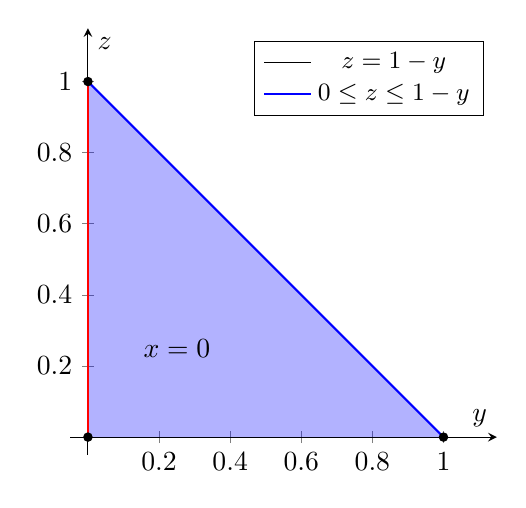
\begin{tikzpicture}
\begin{axis}[
    axis lines=middle,
    xlabel={$y$}, ylabel={$z$},
    xmin=-0.05, xmax=1.15, ymin=-0.05, ymax=1.15,
    domain=0:1, samples=200,
    width=7cm, height=7cm,
    legend pos=north east,
    legend style={font=\small},
]
\addplot[name path=A, draw=none, domain=0:1] {0};
\addplot[name path=B, blue, thick, domain=0:1] {1-x};
\addlegendentry{$z=1-y$}
\addplot[blue, opacity=0.3] fill between[of=A and B];
\addlegendentry{$0\le z\le 1-y$}
\draw[red, thick] (axis cs:0,0) -- (axis cs:0,1);
\draw[red, thick] (axis cs:0,0) -- (axis cs:0,1);
\filldraw (axis cs:0,0) circle (1.5pt);
\filldraw (axis cs:1,0) circle (1.5pt);
\filldraw (axis cs:0,1) circle (1.5pt);
\node at (axis cs:0.25,0.25) {$x=0$};
\end{axis}
\end{tikzpicture}
\end{document}